\documentclass{article}
\usepackage[utf8]{inputenc}
\usepackage{amsmath, amssymb, amsthm}
\usepackage{graphicx, float}
\graphicspath{ {./imagens/} }
\usepackage{multicol}
\usepackage[brazil]{babel}
\usepackage{pgfplots}
\pgfplotsset{compat=1.18}
\usepackage[letterpaper, top = 1in, bottom = 1.0 in, left = 1.2 in, right = 1.2 in, heightrounded]{geometry}

%%%%%%%%%%%%%%%%%%%%%%%%% Caso haja dúvidas na Symbologia %%%%%%%%%%%%%%%%
% https://detexify.kirelabs.org/classify.html
%%%%%%%%%%%%%%%%%%%%%%%%% Parâmetros de construção %%%%%%%%%%%%%%%%%%%%%%%
\setlength{\parindent}{0pt}
\setlength{\parskip}{0.8em}

\title{\textbf{Repositório de Estatistica e Probabilidade}}
\author{UFSC Joinville - EMB5010 \\ Artur Gemaque}
\date{\today}
%%%%%%%%%%%%%%%%%%%%%%%%%% COMEÇO DO DOCUMENTO %%%%%%%%%%%%%%%%%%%%%%%%%%%
\begin{document}
\maketitle

\begin{abstract}
Este documento tempo como principal funcionalidade registrar os contudos ensinados 
em sala de aula pelo professor Jaimes, ademais servirá como fonte de estudo para as 
provas referentes há Matéria.
\end{abstract}

\begin{multicols}{2} % Início da seção com duas colunas
\section{ Estatistica}

      Vamos começar com as definições mais simplórias da matéria que são resultado do cálculo dos dados.

      \subsection{Média}
      A média aritmética de um conjunto de n números é a soma desses números dividida por n.
        \begin{center}
          $ \overset{\_}{x} =  \overset{n}{\underset{i=1}{\sum}} \frac{X_i}{n}  $
        \end{center}

      \subsection{Variância}
      A variância é um conceito fundamental em estatística que mede a dispersão de um conjunto de dados em relação à sua média.
        \begin{center}
          $ (S)^2 =  \frac{\overset{n}{\underset{i=1}{\sum}} (X_i - \overset{\_}{x} )^2 }{n - 1} $
        \end{center}

      \subsection{Desvio padrão}
      O desvio padrão é uma medida de dispersão estatística que indica o quão afastados os 
      dados de um conjunto estão da sua média. Ele é a raiz quadrada da variância, o que o 
      torna mais interpretável.
        \begin{center}
          $ S = \sqrt[2]{S^2}$
        \end{center}

      \subsection{Valores de análise}
      Partindo agora para valores que são obtidos apartir dos dados ordenados em formato crescente. 
      Observação que as seguintes fórmulas serão para que possamos obter as posição dos referidos valores.    
    
      \subsubsection{Mediana}
      Mediana é o número no centro de um grupo de números.
      \begin{center}
        $ Md = X_{(\frac{n + 1}{2})} $
      \end{center}
    
      \subsubsection{Quartis}
      Os quartis são valores que dividem uma amostra de dados em quatro partes iguais e são usados para 
      avaliar a dispersão e a tendência central de um conjunto de dados. Eles são os valores contidos nas 
      posições de $ n*25\% $ entre outras porcentagens, caso "n" dê um valor quebrado o Quartil vai ser a 
      média entre os dois valores.
      \begin{center}
        $ Q_1 = X_{(\frac{n + 1}{4})} $ \\
        $ Q_3 = X_{(\frac{3(n + 1)}{4})} $
      \end{center}

      \subsubsection{Moda}
      A moda é o valor que mais aparece em um conjunto de dados, ou seja, o valor que tem maior frequência.

      \subsubsection{Amplitude}
      A amplitude de um conjunto de dados é a diferença entre o maior e o menor valor. Para calcular a amplitude, 
      subtrai-se o menor valor do maior. 
  
      \subsection{Histograma}
        Um histograma é uma espécie de gráfico de barras que demonstra uma distribuição de frequências. No histograma, 
      a base de cada uma das barras representa uma classe e a altura representa a quantidade ou frequência absoluta com 
      que o valor de cada classe ocorre.
      
      \hbox{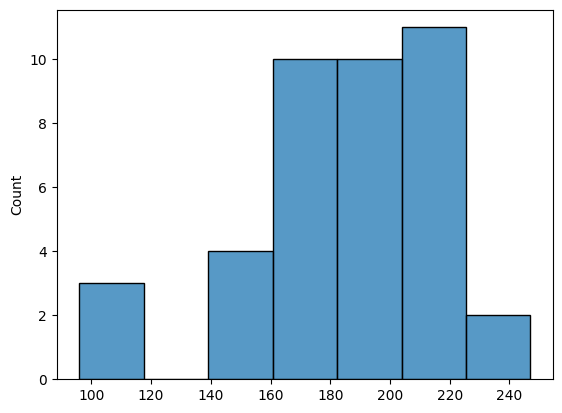
\includegraphics[width=7cm]{Histograma.png}}
      
      \subsection{Boxplot}  
      O Box Plot, que estudamos no curso Green Belt, é uma ferramenta gráfica que ajuda a identificar a existência de 
      possíveis outliers no conjunto de dados. Em um boxplot são apresentadas 5 estatísticas: o mínimo, o primeiro quartil 
      (Q1), a mediana, o terceiro quartil (Q3) e o máximo.
      
      \hbox{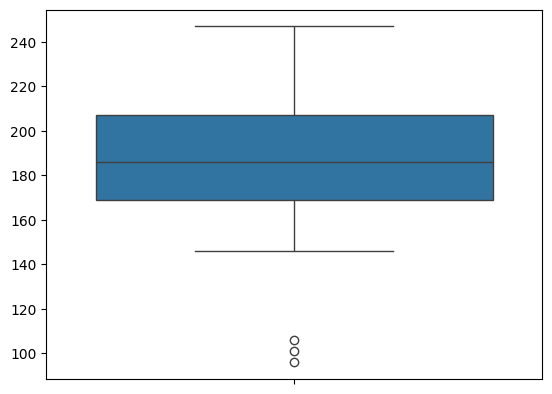
\includegraphics[width=7cm]{Boxplot.png}}  
        
\section{Axiomas da Probabilidade}

    \ Sejam $ A_i $ num espaço amostral $ \Omega: $

    \begin{enumerate}
      \item $ 0 \leqslant P(A_i) \leqslant 1 $
      \item $ P(\Omega) = 1 $
      \item $ P(A_1 \bigcup A_2) = P(A_1) + P(A_2)\\ \Leftrightarrow P(A_1 \cap A_2) = 0 $
    \end{enumerate}

    \ Algumas propriedades decorrentes dos axiomas:
    \begin{list}{ - }{spacing}
      \item $ P( \varnothing ) = 0 $
      \item $ P(A) + P(\overset{\_}{A}) = 1 \ \rightarrow P(\overset{\_}{A}) = 1 - P(A) $
      \item $ P(A_1 \bigcup A_2) = P(A_1) + P(A_2) - P(A_1 \cap A_2) $
    \end{list}
  \end{multicols} % Fim da seção com duas colunas
\newpage

    \subsection{Teorema da Probabilidade Total e Teorema de Bayes}

    \begin{quote}
      Exemplo 1
    \end{quote}

    Um indivíduo possui 3 contas de e-mail diferentes. 
    \begin{multicols}{2}
      
    Do total de mensagens que ele recebe:
    
    \begin{itemize}
      \item 70\% na conta 1
      \item 20\% na conta 2
      \item 10\% na conta 3
    \end{itemize}

    Mensagens que são SPAM

    \begin{itemize}
      \item 1\% das  mensagens da conta 1 
      \item 2\% das  mensagens da conta 2
      \item 5\% das  mensagens da conta 3
    \end{itemize}
    \end{multicols}

    Questão:

    \begin{quote}
      1. Qual a Probabilidade de uma mensagem selecionada aleatoriamente ser SPAM ?
    \end{quote}
      
    Partindo que $ C_1 $ representa a probabilidade de uma mensagem chegar na conta 1 e $ S_1 $ a probabilidade de receber SPAM
    \begin{center}
    \begin{itemize}
      \item $ P(S) = [ C_1 \bigcap S ]\  \bigcup  \ [ C_2 \bigcap S ]\  \bigcup \ [ C_3 \bigcap S ]  $
      \item $ P(S) = P( C_1 \bigcap S ) + P( C_2 \bigcap S ) + P( C_3 \bigcap S )  $
      \item $ P(S) = P(C_1) P( \frac{S}{C_1} ) + P(C_2) P( \frac{S}{C_2} ) + P(C_3) P( \frac{S}{C_3} ) $
      \item $ P(S) = (0,7)*(0,01) + (0,2)*(0,02) + (0,1)*(0,05) $
      \item $ P(S) = 0,0160 \rightarrow 1,6\% $ De se receber um SPAM.
    \end{itemize}
    \end{center}

    \begin{quote}
      2. Sabendo que uma mensagem selecionada aleatoriamente é SPAM qual a probabilidade de que
      ela tenha sido recebida pela conta 3? 
    \end{quote}

    Primeiro redusimos nosso espaço amostral para as mensagens SPAM $ 1,6\% $ e ultilizamos a definição
    de probabilidade 

    \begin{center}
      \begin{large}
        $ P(\frac{C_3}{S}) = \frac{P(C_3 \bigcap S)}{P(S)} \rightarrow  \frac{10\% * 5\%}{1,6\%} = 31,25\% $
      \end{large}
      \end{center}

    Portanto, a probabilidade total é determinada apartir da fórmula
    
    \begin{center}
          $ P(S) = P(E_1) P( \frac{F}{E_1}) + P(E_2) P( \frac{F}{E_2}) + \dots + P(E_k) P( \frac{F}{E_k})  $
    \end{center}

    \newpage
    
    \begin{quote}
      Exemplo 2
    \end{quote}

    Uma doença "rara" acontece 1 em 1000 adultos. Um teste diagnóstifico foi desenvolvido,
    o qual tem o seguinte desempenho:

    \begin{itemize}
      \item Se o indivíduo testado tiver a doença, o teste resulta positivo 99\% das vezes
      \item Se o indivíduo testado \textbf{Não} tiver a doença, o teste resulta positivo 2\% das vezes
    \end{itemize}

    Questão

    \begin{quote}
      1. Se um indivíduo selecionado aleatoriamente foi testado, e o resultado for positivo, qual a 
      probabilidade de ele de fato ter a doença?
    \end{quote}

    Faz ae!

    \begin{center}
    $ P(p) = 4,72\% $ resultado!
    \end{center}
  
    \subsection{Variável Aleatória}

      
    
  
  %\begin{tikzpicture}
  %  \begin{axis}
  %    \addplot3[surf, samples = 20, shader = interp]{1-x^2-y^2};
  %  \end{axis}
  % \end{tikzpicture}


\end{document}